% Created 2022-06-15 Wed 13:42
% Intended LaTeX compiler: pdflatex
\documentclass[11pt]{article}
\usepackage[utf8]{inputenc}
\usepackage[T1]{fontenc}
\usepackage{graphicx}
\usepackage{grffile}
\usepackage{longtable}
\usepackage{wrapfig}
\usepackage{rotating}
\usepackage[normalem]{ulem}
\usepackage{amsmath}
\usepackage{textcomp}
\usepackage{amssymb}
\usepackage{capt-of}
\usepackage{hyperref}
\author{Svoronos - Kanavas Iason}
\date{\today}
\title{Construction sites SonVis Algorithm documentation}
\hypersetup{
 pdfauthor={Svoronos - Kanavas Iason},
 pdftitle={Construction sites SonVis Algorithm documentation},
 pdfkeywords={},
 pdfsubject={},
 pdfcreator={Emacs 27.1 (Org mode 9.0.6)},
 pdflang={English}}
\begin{document}

\maketitle
\tableofcontents


\section{Algorithm architecture}
\label{sec:org71f9984}
The overall algorithm is structured as:
\begin{enumerate}
\item Interface
\item Sub-processes
\item data processing algorithm
\begin{enumerate}
\item outlier identification,
\item replacement,
\item data-frame creation and manipulation,
\item min-max extraction script
\item datetime re-sample function
\end{enumerate}
\item on-run functions (includes matrix printing functions)
\item IPC inter-process communication (\& connection setup functions)
\item Sonification algorithm
\begin{enumerate}
\item processing functions
\item data receiver -- handler
\item synth and data parameter dictionary
\item event receiver - actions
\item IPC connection configuration
\item synthesisers
\item map to scale frequency mapping patch
\end{enumerate}
\end{enumerate}

\section{Dependencies}
\label{sec:org897db6e}
SuperCollider (sclang has to be in \$PATH)

Python \&
Python packages:

from \uline{\uline{future}} import print\(_{\text{function}}\)
import datetime as dt
import panel as pn
import param  \# for FormatDateRangeSlider
import subprocess  \# to run SC
import threading  \# stop iteration cycle when kill button pressed
\#from pythonosc import udp\(_{\text{client}}\)
from bokeh.models import Slider, CheckboxGroup, CustomJS, Label
import os
import numpy as np
import pandas as pd
import time
import datetime
from dateutil import parser
from pythonosc import udp\(_{\text{client}}\)
import subprocess
import numpy as np
import pandas as pd
import matplotlib.pyplot as plt
import random
import sys
from bokeh.plotting import figure
from pythonosc.osc\(_{\text{server}}\) import AsyncIOOSCUDPServer
from pythonosc.dispatcher import Dispatcher
import asyncio

\section{Interface}
\label{sec:orgacf52b9}
The interface consists of certain visual elements.
The datetime range slider and text input (for the time) are used for date and time accordingly. Using these the user can specify a desired datetime period in the data to sonify and visualise.

\begin{center}
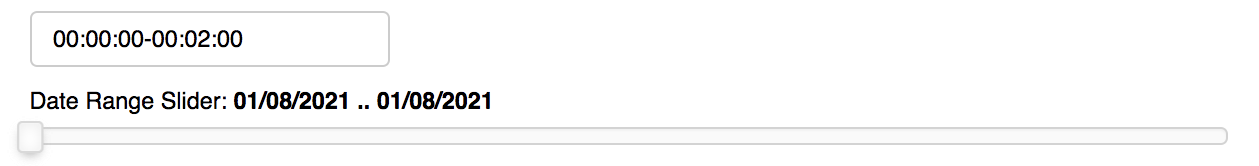
\includegraphics[width=.9\linewidth]{./datetime_selection.png}
\end{center}

The \textbf{start} button is used so that the datetime period is extracted and then sent to be sonified and visualised, while the \textbf{killall} button can interrupt/stop every running procedure in relation to the sonification and visualisation process anytime.

\begin{center}
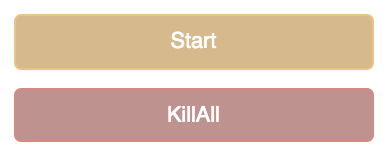
\includegraphics[width=.9\linewidth]{./start_kill_buttons.png}
\end{center}

Below, there is a checkbox where the user can select the period of the values in the data to re-sample.

\begin{center}

\includegraphics[width=.9\linewidth]{./resample_checkbox.png}
\end{center}

The original collection period is (every) 30 seconds.  The re-sample options are, per minute (T), per 30 minutes (30M), per hour (H), per week (W), per month (M).  In the re-sample function (see below), the data values are derived in every period with selecting the max value when doing the frequency conversion to highlight peaks in the data.  For example, if we want to re-sample with 1 minute re-sample frequency (T). We have initially:
\begin{center}
\begin{tabular}{lr}
\hline
timestamp, & data\\
2021-08-01 00:00:00, & 2\\
2021-08-01 00:00:30, & 0\\
2021-08-01 00:01:00, & 4\\
\hline
\end{tabular}
\end{center}

Re-sample result: The extracted value for the first minute will be "4" because is the max value observed for this minute.

Then, there is a another slider that controls the data iteration frequency and it has a range from 1 to 1000 values per second.

\begin{center}
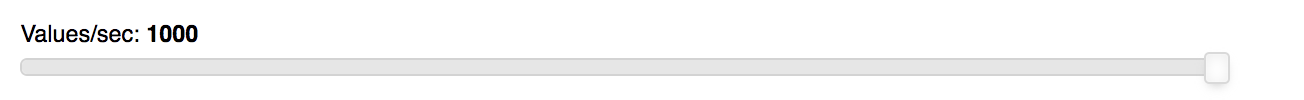
\includegraphics[width=.9\linewidth]{./values_sec.png}
\end{center}

Finally, there are six buttons where the user can use to turn on/off, the desired data parameters to sonify - visualise

\begin{center}
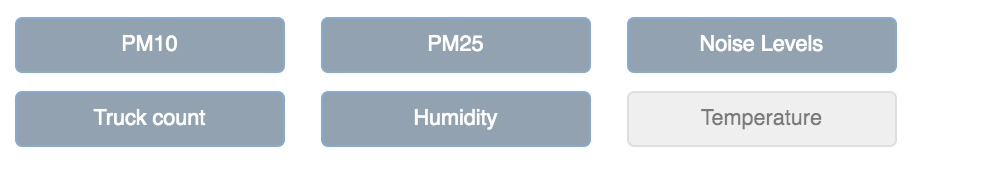
\includegraphics[width=.9\linewidth]{./synth_onoff.png}
\end{center}

\vspace{0.5em}

Overall, the button python bokeh elements, trigger osc messages that are sent from python to supercollider in order to control different synths.
The ones that utilise this functionality is the \textbf{start} \textbf{killall} and the synth on/off buttons (pm10, pm25, temp, humidity, noise levels, truck count).
This will be elaborated in the IPC section

\section{Sub-processes}
\label{sec:orgd727bb3}
On launch, sclang is initialised and runs as a sub-process within the python session.  More specifically, the SuperCollider  patch for sonification is evaluated using the following command in Python.
\begin{verbatim}
# run sonification patch
sclang = subprocess.Popen(
    'sclang particleSonification.scd', shell=True,
    stdout=subprocess.PIPE,
    stderr=subprocess.STDOUT)
\end{verbatim}
Getting back now to the initialisation python script where a function obtains the IP address of the computer using a shell command and then stores it as a global variable.  After that, the OSC client configuration setup uses the variable's value (udp\(_{\text{client}}\) object).  The function is defined the following way as well as the OSC setup.  This process easily configures OSC intercommunication between python and SuperCollider therefore mistakes and hassle by hard-coding IP addresses or manual configurations are avoided.

\begin{verbatim}
# get IP address
def getip():
    global ip
    ip = subprocess.Popen(
        'ipconfig getifaddr en0', shell=True,
        stdout=subprocess.PIPE,
        stderr=subprocess.STDOUT)
    ip, _ = ip.communicate()
    ip = ip.decode('utf-8')
    ip = ip.strip()
    print(ip)

# Python osc
getip() # run getip function
client = udp_client.SimpleUDPClient(ip, 57120)
\end{verbatim}
\textbf{Note:} \emph{this works \textbf{only for macOs}.  Therefore it has to be adjusted for linux or windows.}

\vspace{0.2cm}
\noindent
WIN hint:
\begin{verbatim}
ipconfig | grep IPv4 Address.
\end{verbatim}

\section{data processing}
\label{sec:org0414196}
In this section the data processing will be described.  The algorithm is developed in Python.  The idea is based on combining and re-constructing the data-sets after the processing results that come out from the derived stats (IQR).  SC has also access to the derived data-set (it is written to disk) so that it has access to the min max values for the correct mapping (see \ref{sec:org206d8c7}).  In this way, it is also possible to re-use the algorithm with different data since the mapping is not hard-coded.

Outlier identification and replacement was deemed necessary since it was observed by using box-plot stats the PM (both 25 and 10) showed extreme values (far from accurate measurements (140\textasciitilde{} PM10) ) that we would like to exclude.

\begin{center}
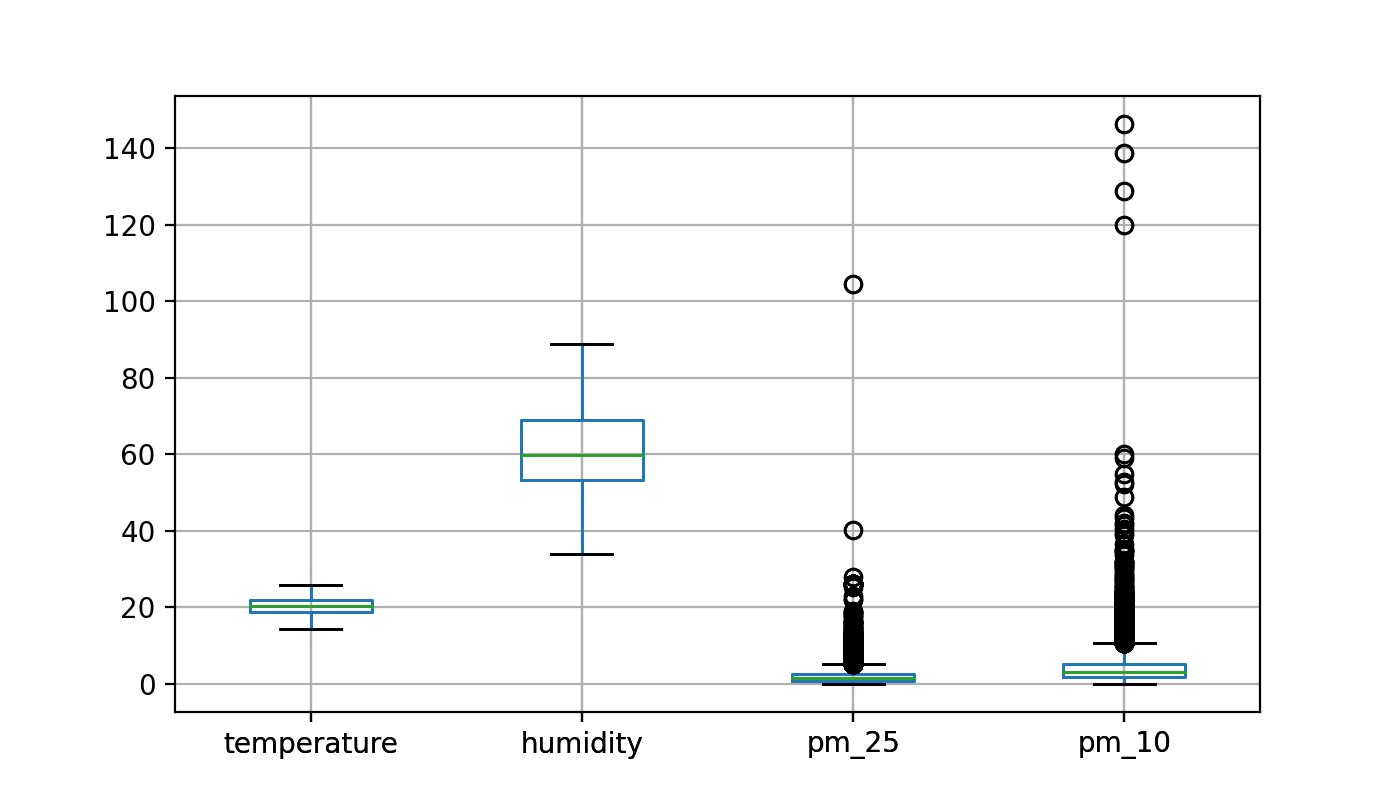
\includegraphics[width=.9\linewidth]{./boxplot.png}
\end{center}

Code process:

The very first step is that the original data are loaded from the CSV file while the timestamp column is stored in a variable.  Then the timestamp column is removed from the data-set to do the processing and then added again in the very end of the procedure.

\subsection{outlier identification}
\label{sec:orgb74fda1}
Descriptive statistics are applied in the data-set using the 'describe()' method from pandas.  That is to calculate percentiles, max, min and mean of every column in the data-set.  Then the Q1 and Q3 of PM10 and PM25 are stored in variables.  The IQR of both is calculated as well as the max and min threshold.  The threshold will be used to identify the outliers.  Values that exceed the min and max threshold are the outliers.

\begin{verbatim}
# calculate IQRange for pm_25 from q1 and q3
iqr_pm25 = pm25_q3-pm25_q1
iqr_pm10 = pm10_q3-pm10_q1

# calculate thresholds from IQR -- acc. skewed distribution
# max_thresh: Q3+1.5IQR
# min_thresh: Q1-1.5IQR
max_thresh_pm_25 = pm25_q3+(1.5*iqr_pm25)
min_thresh_pm_25 = pm25_q1-(1.5*iqr_pm25)
max_thresh_pm_10 = pm10_q3+(1.5*iqr_pm10)
min_thresh_pm_10 = pm10_q1-(1.5*iqr_pm10)
thresholds = {'min thresh_pm_25': min_thresh_pm_25,
         'max thresh_pm_25': max_thresh_pm_25,
         'min thresh_pm_10': min_thresh_pm_10,
         'max thresh_pm_10': max_thresh_pm_10}
\end{verbatim}

\subsection{replacement}
\label{sec:org0d6c451}
Values for PM10 and PM25 that exceeded min and max threshold derived from the IQR calculation will be NaN-ed and then replaced with randomly selected samples from the same column in the data-set.  This outlier replacement process takes place for PM10, PM25 and noise levels.  The replacement function also prints how many values were replaced.

\begin{verbatim}
def replaceOutliers(col,minimum_thres,maximum_thres):
    for i in [col]: # replace outliers with nan value
        min = minimum_thres
        max = maximum_thres
        df.loc[df[i] < min, i] = np.nan  # if value is < min_thresh_pm25: nan it
        df.loc[df[i] > max, i] = np.nan  # if value is > max_thresh_pm25: nan it
        df.loc[df[i] == 0, i] = 0.1  # if zero: replace it with 0.1 (smallest val)
        print( # print how many null values are in the specified column
            'sum of null replaced values',
            df[col].isnull().sum())
        global des_col
        des_col = [col] # specify column
\end{verbatim}

\begin{verbatim}
df = df.apply( # replace NaN values from random samples same column
    lambda x: np.where(x.isnull(), x.dropna().sample(len(x), replace=True), x))
\end{verbatim}

\subsection{data-frame creation and manipulation}
\label{sec:org354e853}
As mentioned the df is first loaded from the CSV file, while the timestamp column is removed and stored in a variable.  This was done to easily process the data-set without interfering with the datetime object (timestamp column).  After that the \ref{sec:orgb74fda1} takes place.  That results to a new data-frame and then the timestamp column is added (insert method).
\begin{verbatim}
# insert timestamp column
df.insert(0, "timestamp", timestamp, True)
\end{verbatim}

Afterwards, the noise level data are loaded and stored in a variable.  The last (cat\(_{\text{24}}\)) column was used.  This column is added to the data-frame that contains everything.  While in the next step the replaceOutliers function is applied to the noise levels column as well ('db').  The threshold that was used aimed to exclude one outlier (5.444976) that was identified by rendering a boxplot from the column data.

Then the truck\(_{\text{count}}\) data are inserted to the main data-frame after the appropriate data processing that is related to the ';' delimiter character splitting. This was done using the pandas data-frame loading process.

\begin{verbatim}
trucks_df = pd.read_csv(  # read truck data file
    "./fake_passage_time.csv",
    delimiter=';')
\end{verbatim}

After that the main data-frame is written to disk within a certain directory path in the current working directory environment.  That would be the \url{./df\_out} directory.
Later the data-frame is registered to a global variable for easier access.

\subsection{min-max extraction script}
\label{sec:org206d8c7}
The min-max python script was used for use within SuperCollider.  Its purpose is to run the min and max basic python methods to certain columns.  These values will be used for the paramenter mapping.  It returns the min and max value of the specified column.  These are stored in a dictionary.  More information can be found at  \ref{sec:org13f233f}.

It takes 2 arguments, these are:
\begin{enumerate}
\item data-file that the min max values will be extracted
\item column in the data-set
\end{enumerate}

It runs from the terminal with the following command.
\begin{verbatim}
python minmax.py data-file column
\end{verbatim}

In SuperCollider this command will run using the "unixCmdGetStdOutLines" method.  It will return the values as "string" in the SuperCollider environment.

\subsection{datetime re-sample function}
\label{sec:orgb480f41}
\textbf{Not 100\% implemented}

This function was implemented to re-sample the processed data-frame.  In the non-resampled one the collection frequency is 30s. So, every 30 seconds a new value is stored for all parameters.

While this can of course result to precise estimations regarding events in the data it might not be very convenient if someone would like to quickly listen longer time periods.  For example, with an iteration frequency of 1000 values per second it takes 86.4 seconds time to listen to one day.  This was thought as a limitation and that's why this function was implemented to create down-sampled versions of the main data-set.  Speeding up the iteration frequency was not an option because of computing power limitations.

The frequencies in the re-sampling process that was selected are:
\begin{enumerate}
\item 30S (non re-sampled)
\item T / 1 minute
\item 30M / 30 minutes
\item H / 1 Hour
\item D / 1 Day
\item W / 1 Week
\item M / 1 Month
\end{enumerate}

The re-sample function is accessed by the checkbox on the interface \ref{sec:orgacf52b9}.  In every re-sample period the maximum value observed is stored.  For example, the non re-sampled data-set has:

\begin{center}
\begin{tabular}{rr}
\hline
00:00:00 & 0\\
00:00:30 & 1\\
00:01:00 & 4\\
\hline
\end{tabular}
\end{center}

If the re-sampling frequency is T (1 min) the 4 value will be stored in this cycle.

\begin{center}
\begin{tabular}{rr}
\hline
00:00:00 & 4\\
\hline
\end{tabular}
\end{center}

Overall, the re-sample function is base on the resample() method in combination with certain conditional tasks so that the correct checkbox element corresponds to the according resample function parameters.  Technically, it is actually divided into two functions.  The first does the conditional argument setting (feeds the correct arguments to the other function) while the other does the actual re-sampling and writes it to disk (CSV).

In the iteration process \ldots{} \textbf{TO BE DONE \& REPORTED}  (Write only re-sampling function related info, next section is: on-run functions)

\section{on-run functions}
\label{sec:org66ce3ff}
\section{IPC inter-process communication (includes connection setup functions)}
\label{sec:org5c532d5}
The IPC is based on the OSC protocol and its aim is to interconnect Python and SueprCollider.  It is based on sending individual messages from the Python process triggered by the Python interface elements.

In the OSC configuration there are 3 different OSC addresses that allow communication between the two software.  These are:
\begin{enumerate}
\item \label{org626b5a6} | main address for the iteration process.  SC received the data values (OSCdef).  Py → SC
\item \label{org92feb10} | controls the synths, acts like an ON/OFF switch.  Triggered by the 6 synth ON/OFF buttons. Py → SC
\item \label{org2c5d731} | This acts like main ON/OFF switch for the all synths, it is triggered by the START and Killall buttons. Py → SC
\item \label{org1654376} | Initialisation address, activates the interaction elements on the interface when (or if) the SC responds.  This configuration uses the 1234 port instead. SC → Py
\end{enumerate}

The initial configuration is related to obtaining the IP address of the computer automatically to avoid manual configurations.  This was implemented with the following functions in Python and SuperCollider.

\textbf{Python}

\begin{verbatim}
# get IP address
def getip():
    global ip
    ip = subprocess.Popen(
        'ipconfig getifaddr en0', shell=True,
        stdout=subprocess.PIPE,
        stderr=subprocess.STDOUT)
    ip, _ = ip.communicate()
    ip = ip.decode('utf-8')
    ip = ip.strip()
    print(ip)


# Python osc
getip() # run getip function
client = udp_client.SimpleUDPClient(ip, 57120)
\end{verbatim}

To simplify, this function runs
\begin{verbatim}
'ipconfig getifaddr en0'
\end{verbatim}
in the terminal and extracts the current ip address, stores it in a variable and uses it for the OSC UDP client setup.

\textbf{SuperCollider}

On the SC side now the configuration is implemented in the following way
\begin{verbatim}
~ip = ("ipconfig getifaddr en0").unixCmdGetStdOutLines[0]; // get ip
n = NetAddr(~ip, 1234); // set netaddress
n.sendMsg('/startup/',1); // send to python that everything is loaded to enable buttons
("python communication established").postln;
\end{verbatim}

At this point where the above command runs, an OSC message is sent to python using the '\emph{startup}' address.  In the OSC server function (receiver) in Python a task activates the interaction elements on the interface.  This process can be found in the oscServerPython.scd file \url{../src/oscServerPython.py}.

The communication using the \ref{org626b5a6} address is the most important one since concerns the iteration process.  The data values in every iteration cycle (row by row) are sent to SuperCollider as shown below.

\begin{verbatim}
client.send_message("/pysc", datetime_selection.iloc[i])
\end{verbatim}
\section{Sonification algorithm}
\label{sec:org13f233f}
\subsection{processing functions}
\label{sec:org4b31ca5}
\subsection{data receiver -- handler}
\label{sec:org5ab6084}
\subsection{synth and data parameter dictionary}
\label{sec:org58a921a}
Speak about the mapping (max-min values py script).  Mentioned at \ref{sec:org206d8c7}
\begin{verbatim}
com =  ("python"+(~path+/+"minmax.py").standardizePath+(~path+/+file)+col).unixCmdGetStdOutLines;
        (~path+/+file).postln;
\end{verbatim}
\subsection{event receiver - actions}
\label{sec:orgfa0cea3}
\subsection{IPC connection configuration}
\label{sec:orgcc09955}
\subsection{synthesisers}
\label{sec:orgb25d361}
\subsection{map to scale frequency mapping patch}
\label{sec:orga1cbe34}
\end{document}
